\documentclass{vkr}
\usepackage[english, russian]{babel} % переносы
\usepackage{graphicx} % для вставки картинок
\graphicspath{{images/}} % путь к изображениям
\usepackage[hidelinks]{hyperref}
\usepackage{float} % определяет метод H для рисунка с переносом на следующую страницу, ели не помещается
\usepackage{pdflscape}
\addto{\captionsrussian}{\renewcommand{\refname}{СПИСОК ИСПОЛЬЗОВАННЫХ ИСТОЧНИКОВ}}
\usepackage{xltabular} % для вставки таблиц
\usepackage{makecell}
\renewcommand\theadfont{} % шрифт в /thead
\usepackage{array} % для определения новых типов столбцов таблиц
\newcolumntype{T}{>{\centering\arraybackslash}X} % новый тип столбца T - автоматическая ширина столбца с выравниванием по центру
\newcolumntype{R}{>{\raggedleft\arraybackslash}X} % новый тип столбца R - автоматическая ширина столбца с выравниванием по правому краю
\newcolumntype{C}[1]{>{\centering\let\newline\\\arraybackslash\hspace{0pt}}m{#1}} % новый тип столбца C - фиксированная ширина столбца с выравниванием по центру
\newcolumntype{r}[1]{>{\raggedleft\arraybackslash}p{#1}} % новый тип столбца r - фиксированная ширина столбца с выравниванием по правому краю
\newcommand{\centrow}{\centering\arraybackslash} % командой \centrow можно центрировать одну ячейку (заголовок) в столбце типа X или p, оставив в оcтальных ячейках другой тип выравнивания
\newcommand{\finishhead}{\endhead\hline\endlastfoot}
\newcommand{\continuecaption}[1]{\captionsetup{labelformat=empty} \caption[]{#1}\\ \hline }
\usepackage{etoolbox}
\AtBeginEnvironment{xltabular}{\refstepcounter{tablecnt}} % подсчет таблиц xltabular, обычные таблицы подсчитываются в классе

\usepackage[tableposition=top]{caption} % подпись таблицы вверху
\captionsetup{strut=off}
\setlength{\intextsep}{0pt} % Vertical space above & below [h] floats
\setlength{\textfloatsep}{0pt} % Vertical space below (above) [t] ([b]) floats
\DeclareCaptionLabelFormat{gostfigure}{Рисунок #2} %подпись рисунка
\DeclareCaptionLabelFormat{gosttable}{Таблица #2} %подпись таблицы
\DeclareCaptionLabelSeparator{gost}{~--~} %разделитель в рисунках и таблицах
\captionsetup{labelsep=gost}
\captionsetup[figure]{aboveskip=10pt,belowskip=4mm,justification=centering,labelformat=gostfigure} % настройка подписи рисунка
\captionsetup[table]{font={stretch=1.41},skip=0pt,belowskip=0pt,aboveskip=8.5pt,singlelinecheck=off,labelformat=gosttable} % настройка подписи таблицы

\setlength{\LTpre}{8mm} % отступ сверху таблицы
\setlength{\LTpost}{6mm} % отступ снизу таблицы

\usepackage{enumitem}
\setlist{nolistsep,wide=\parindent,itemindent=*} % отступы вокруг списков, выравнивание с учетом разделителя

\usepackage{color} %% это для отображения цвета в коде
\usepackage{listings} %% листинги кода
\setmonofont[Scale=0.7]{Verdana} % моноширный шрифт для листинга

\definecolor{codegreen}{rgb}{0,0.6,0}
\definecolor{codegray}{rgb}{0.5,0.5,0.5}
\definecolor{codepurple}{rgb}{0.58,0,0.82}

\lstset{ %
language=C,                 % выбор языка для подсветки (здесь это С)
numbers=left,               % где поставить нумерацию строк (слева\справа)
numberstyle=\tiny,           % размер шрифта для номеров строк
stepnumber=1,                   % размер шага между двумя номерами строк
numbersep=5pt,                % как далеко отстоят номера строк от подсвечиваемого кода
commentstyle=\color{codegreen},
keywordstyle=\color{magenta},
numberstyle=\tiny\color{codegray},
stringstyle=\color{codepurple},
basicstyle=\linespread{0.95}\ttfamily,
backgroundcolor=\color{white}, % цвет фона подсветки - используем \usepackage{color}
showspaces=false,            % показывать или нет пробелы специальными отступами
showstringspaces=false,      % показывать или нет пробелы в строках
showtabs=false,             % показывать или нет табуляцию в строках
frame=single,              % рисовать рамку вокруг кода
tabsize=2,                 % размер табуляции по умолчанию равен 2 пробелам
captionpos=t,              % позиция заголовка вверху [t] или внизу [b] 
breaklines=true,           % автоматически переносить строки (да\нет)
breakatwhitespace=false, % переносить строки только если есть пробел
escapeinside={\%*}{*)}   % если нужно добавить комментарии в коде
}

\makeatletter % чтобы допускались русские комментарии в листингах
\lst@InputCatcodes
\def\lst@DefEC{%
 \lst@CCECUse \lst@ProcessLetter
  ^^80^^81^^82^^83^^84^^85^^86^^87^^88^^89^^8a^^8b^^8c^^8d^^8e^^8f%
  ^^90^^91^^92^^93^^94^^95^^96^^97^^98^^99^^9a^^9b^^9c^^9d^^9e^^9f%
  ^^a0^^a1^^a2^^a3^^a4^^a5^^a6^^a7^^a8^^a9^^aa^^ab^^ac^^ad^^ae^^af%
  ^^b0^^b1^^b2^^b3^^b4^^b5^^b6^^b7^^b8^^b9^^ba^^bb^^bc^^bd^^be^^bf%
  ^^c0^^c1^^c2^^c3^^c4^^c5^^c6^^c7^^c8^^c9^^ca^^cb^^cc^^cd^^ce^^cf%
  ^^d0^^d1^^d2^^d3^^d4^^d5^^d6^^d7^^d8^^d9^^da^^db^^dc^^dd^^de^^df%
  ^^e0^^e1^^e2^^e3^^e4^^e5^^e6^^e7^^e8^^e9^^ea^^eb^^ec^^ed^^ee^^ef%
  ^^f0^^f1^^f2^^f3^^f4^^f5^^f6^^f7^^f8^^f9^^fa^^fb^^fc^^fd^^fe^^ff%
  ^^^^20ac^^^^0153^^^^0152%
  % Basic Cyrillic alphabet coverage
  ^^^^0410^^^^0411^^^^0412^^^^0413^^^^0414^^^^0415^^^^0416^^^^0417%
  ^^^^0418^^^^0419^^^^041a^^^^041b^^^^041c^^^^041d^^^^041e^^^^041f%
  ^^^^0420^^^^0421^^^^0422^^^^0423^^^^0424^^^^0425^^^^0426^^^^0427%
  ^^^^0428^^^^0429^^^^042a^^^^042b^^^^042c^^^^042d^^^^042e^^^^042f%
  ^^^^0430^^^^0431^^^^0432^^^^0433^^^^0434^^^^0435^^^^0436^^^^0437%
  ^^^^0438^^^^0439^^^^043a^^^^043b^^^^043c^^^^043d^^^^043e^^^^043f%
  ^^^^0440^^^^0441^^^^0442^^^^0443^^^^0444^^^^0445^^^^0446^^^^0447%
  ^^^^0448^^^^0449^^^^044a^^^^044b^^^^044c^^^^044d^^^^044e^^^^044f%
  ^^^^0401^^^^0451%
  %%%
  ^^00}
\lst@RestoreCatcodes
\makeatother


% Режим шаблона (должен быть включен один из трех)
%\ВКРtrue
\Практикаtrue
%\Курсоваяtrue

\newcommand{\Дисциплина}{<<Проектирование и архитектура программных систем>>} % для курсовой
\newcommand{\КодСпециальности}{09.03.04} % Курсовая
\newcommand{\Специальность}{Программная инженерия} % Курсовая
\newcommand{\Тема}{Разработка web-сайта «Русатом – Аддитивные технологии» на платформе} % ВКР Курсовая
\newcommand{\ТемаВтораяСтрока}{1С-Битрикс}
\newcommand{\ГдеПроводитсяПрактика}{Юго-Западном государственном университете} % для практики
\newcommand{\РуководительПрактПредпр}{Федосов Д. В.} % для практики
\newcommand{\ДолжнРуководительПрактПредпр}{директор} % для практики
\newcommand{\РуководительПрактУнивер}{Чаплыгин А. А.} % для практики
\newcommand{\ДолжнРуководительПрактУнивер}{к.т.н. доцент} % для практики
\newcommand{\Автор}{Б.Р. Якубов}
\newcommand{\АвторРод}{Якубов Б.Р.}
\newcommand{\АвторПолностьюРод}{Якубова Богдана Романовича} % для практики
\newcommand{\Шифр}{21-06-0052}
\newcommand{\Курс}{4} % для практики
\newcommand{\Группа}{ПО-11б}
\newcommand{\Руководитель}{А. А. Чаплыгин} % для ВКР и курсовой
\newcommand{\Нормоконтроль}{А. А. Чаплыгин} % для ВКР
\newcommand{\ЗавКаф}{А. В. Малышев} % для ВКР
\newcommand{\ДатаПриказа}{«07» апреля 2023~г.} % для ВКР
\newcommand{\НомерПриказа}{1505-с} % для ВКР
\newcommand{\СрокПредоставления}{«13» июня 2023~г.} % для ВКР, курсового

\begin{document}
\maketitle
\ifПрактика{}\else{
   \newpage
\begin{center}
\large\textbf{Минобрнауки России}

\large\textbf{Юго-Западный государственный университет}
\vskip 1em
\normalsize{Кафедра программной инженерии}
\vskip 1em
\ifВКР{
        \begin{flushright}
        \begin{tabular}{p{.4\textwidth}}
        \centrow УТВЕРЖДАЮ: \\
        \centrow Заведующий кафедрой \\
        \hrulefill \\
        \setarstrut{\footnotesize}
        \centrow\footnotesize{(подпись, инициалы, фамилия)}\\
        \restorearstrut
        «\underline{\hspace{1cm}}»
        \underline{\hspace{3cm}}
        20\underline{\hspace{1cm}} г.\\
        \end{tabular}
        \end{flushright}
        }\fi
\end{center}
\vspace{1em}
  \begin{center}
  \large
\ifВКР{
ЗАДАНИЕ НА ВЫПУСКНУЮ КВАЛИФИКАЦИОННУЮ РАБОТУ
  ПО ПРОГРАММЕ БАКАЛАВРИАТА}
  \else
ЗАДАНИЕ НА КУРСОВУЮ РАБОТУ (ПРОЕКТ)
\fi
\normalsize
  \end{center}
\vspace{1em}
{\parindent0pt
  Студента \АвторРод, шифр\ \Шифр, группа \Группа
  
1. Тема «\Тема\ \ТемаВтораяСтрока»
\ifВКР{
утверждена приказом ректора ЮЗГУ от \ДатаПриказа\ № \НомерПриказа
}\fi.

2. Срок предоставления работы к защите \СрокПредоставления

3. Исходные данные для создания программной системы:

3.1. Перечень решаемых задач:}

\renewcommand\labelenumi{\theenumi)}

\begin{enumerate}
\item проанализировать IT-инфраструктуру предприятия;
\item  разработать концептуальную модель системы управления IT-ин\-фра\-струк\-турой предприятия на основе подхода к управлению и организации ИТ-услуг ITSM;
\item спроектировать программную систему управления IT-ин\-фра\-струк\-турой предприятия;
\item сконструировать и протестировать программную систему управления IT-инфраструктурой предприятия.
\end{enumerate}

{\parindent0pt
  3.2. Входные данные и требуемые результаты для программы:}

\begin{enumerate}
\item Входными данными для программной системы являются: данные
справочников комплектующих, конфигураций, ПО, критериев качества SLA,
ИТ-услуг, департаментов компании; технические данные ИТ-ресурсов; данные входящих заявок на ИТ-ресурсы; данные запросов поставщикам на комплектующие.
\item Выходными данными для программной системы являются: сформированные заявки на обслуживание ИТ-ресурсов; сформированные запросы на
закупку комплектующих; сведения о выполненных работах по заявкам; статусы заявок; выходные отчеты (инфографика) – по качеству услуг, по состоянию ИТ-ресурсов, по деятельности ИТ-отдела, по стоимости обслуживания
ИТ-ресурсов, воронка заявок.
\end{enumerate}

{\parindent0pt

  4. Содержание работы (по разделам):
  
  4.1. Введение.
  
  4.1. Анализ предметной области.
  
4.2. Техническое задание: основание для разработки, назначение разработки,
требования к программной системе, требования к оформлению документации.

4.3. Технический проект: общие сведения о программной системе, проект
данных программной системы, проектирование архитектуры программной системы, проектирование пользовательского интерфейса программной системы.

4.4. Рабочий проект: спецификация компонентов и классов программной системы, тестирование программной системы, сборка компонентов программной системы.

4.5. Заключение.

4.6. Список использованных источников.

5. Перечень графического материала:

\списокПлакатов

\vskip 2em
\begin{tabular}{p{6.8cm}C{3.8cm}C{4.8cm}}
Руководитель \ifВКР{ВКР}\else работы (проекта) \fi & \lhrulefill{\fill} & \fillcenter\Руководитель\\
\setarstrut{\footnotesize}
& \footnotesize{(подпись, дата)} & \footnotesize{(инициалы, фамилия)}\\
\restorearstrut
Задание принял к исполнению & \lhrulefill{\fill} & \fillcenter\Автор\\
\setarstrut{\footnotesize}
& \footnotesize{(подпись, дата)} & \footnotesize{(инициалы, фамилия)}\\
\restorearstrut
\end{tabular}
}

\renewcommand\labelenumi{\theenumi.}

   \abstract{РЕФЕРАТ}

Объем работы равен \formbytotal{lastpage}{страниц}{е}{ам}{ам}. Работа содержит \formbytotal{figurecnt}{иллюстраци}{ю}{и}{й}, \formbytotal{tablecnt}{таблиц}{у}{ы}{}, \arabic{bibcount} библиографических источников и \formbytotal{числоПлакатов}{лист}{}{а}{ов} графического материала. Количество приложений – 2. Графический материал представлен в приложении А. Фрагменты исходного кода представлены в приложении Б.

Перечень ключевых слов: коммерческий сайт, Система, CMS, Битрикс, Joomla, аддитивные технологии, 3D-принтеры, услуги, сервисы, информатизация, автоматизация, информационные технологии, веб-форма,  Apache, классы, база данных, средства защиты информации, подсистема, компонент, модуль, сущность, информационный блок, метод, контент-редактор, администратор, пользователь, web-сайт.

Объектом разработки является web-сайт компании,  занимающейся производством 3D-принтеров, выпуском оборудования для создания порошков, разработкой программного обеспечения и организацией центров аддитивного производства.

Целью выпускной квалификационной работы является привлечение клиентов, увеличение заказов, информирование о продукции и услугах путем создания сайта компании.

В процессе создания сайта были выделены основные сущности путем создания информационных блоков, использованы классы и методы модулей, обеспечивающие работу с сущностями предметной области, а также корректную работу web-сайта, разработаны разделы, содержащие информацию о компании, ее деятельности, производимой продукции и услугах, разработан сервис по заказу 3D-деталей.

При разработке сайта использовалась система управления контентом "<1С-Битрикс: Управление сайтом">.

Разработанный сайт был успешно внедрен в компании.

\selectlanguage{english}
\abstract{ABSTRACT}
  
The volume of work is \formbytotal{lastpage}{page}{}{s}{s}. The work contains \formbytotal{figurecnt}{illustration}{}{s}{s}, \formbytotal{tablecnt}{table}{}{s}{s}, \arabic{bibcount} bibliographic sources and \formbytotal{числоПлакатов}{sheet}{}{s}{s} of graphic material. The number of applications is 2. The graphic material is presented in annex A. The layout of the site, including the connection of components, is presented in annex B.

List of keywords: commercial website, System, CMS, Bitrix, Joomla, additive technologies, 3D printers, services, services, informatization, automation, information technology, web form, Apache, classes, database, component, module, entity, information block, method, content editor, administrator, user, web site.

The object of the research is the analysis of information technologies for the development of a production company's website.

The object of the development is the website of a company engaged in the production of 3D printers, the production of equipment for the creation of powders, software development and the organization of additive manufacturing centers.

The purpose of the final qualifying work is to attract customers, increase orders, inform about products and services by creating a company website.

In the process of creating the site, the main entities were identified by creating information blocks, classes and methods of modules were used to ensure work with the entities of the subject area, as well as the correct operation of the website, sections containing information about the company, its activities, products and services were developed, a service for ordering 3D parts was developed.

When developing the site, the content management system <<1C – Bitrix: Site Management>> was used.

The developed website was successfully implemented in the company.
\selectlanguage{russian}
}\fi
\tableofcontents
\section*{ОБОЗНАЧЕНИЯ И СОКРАЩЕНИЯ}

БД -- база данных.

ИС -- информационная система.

ИТ -- информационные технологии. 

КТС -- комплекс технических средств.

ОМТС -- отдел материально-технического снабжения. 

ПО -- программное обеспечение.

РП -- рабочий проект.

СУБД -- система управления базами данных.

ТЗ -- техническое задание.

ТП -- технический проект.

UML (Unified Modelling Language) -- язык графического описания для объектного моделирования в области разработки программного обеспечения.

\ifПрактика{}\else{\section*{ВВЕДЕНИЕ}
\addcontentsline{toc}{section}{ВВЕДЕНИЕ}

Современные корпоративные коммуникации требуют специализированных решений, обеспечивающих безопасность данных и эффективное взаимодействие сотрудников. Разработанный закрытый корпоративный мессенджер представляет собой веб-приложение с функциями групповой и приватной переписки, управлением доступом.

Ключевые преимущества решения:
\begin{itemize}
	\item Система аутентификации (логин/пароль)
	\item Ролевое управление группами (модератор/владелец/участник)
	\item Шифрование передаваемых данных (HTTPS)
	\item Поддержка многопользовательских чатов
	\item История сообщений с временными метками
	\item Отправка файлов всех форматов
\end{itemize}

\emph{Цель работы} — создание безопасной платформы для внутренней коммуникации с функциями:
\begin{itemize}
	\item Общий и групповые чаты
	\item Приватная переписка
	\item Управление членством в группах
	\item Поиск по истории сообщений
\end{itemize}

\emph{Задачи исследования}:
\begin{itemize}
	\item Анализ требований к корпоративным коммуникационным системам
	\item Проектирование модульной архитектуры
	\item Реализация серверной части на Python
	\item Создание адаптивного веб-интерфейса
	\item Тестирование безопасности и нагрузки
\end{itemize}}\fi
\section{Анализ предметной области}
\subsection{Современные тенденции корпоративных коммуникаций}

Корпоративные мессенджеры - это специализированные платформы, ориентированные на оптимизацию рабочих процессов. В отличие от массовых сервисов (WhatsApp, Telegram), они предоставляют инструменты для структурированной коммуникации внутри организаций, интеграции с бизнес-приложениями и контроля данных.
Основными функциями корпоративного мессенджера являются:
\begin{itemize}
	\item Обмен сообщениями и файлами
	\item Безопасность и контроль данных
	\item Организация коммуникации
	\item Групповые чаты сотрудников (общие, тематические, отделов, команд)
	\item Личные чаты между сотрудниками
	\item Интеграция с другими сервисами и системами для управления задачами
	\item Управление доступом для пользователей (администратор, модератор, сотрудник, клиент, иной пользователь)
	\item Кроссплатформенность
	\item Встроенная IP-телефония
	\item Таймер автоматического удаления сообщений и файлов
\end{itemize}

На отечественном, так и на зарубежном рынке были успешно представлены такие решения:
\begin{itemize}
	\item Microsoft Teams — глубокая интеграция с экосистемой Microsoft, поддержка многотысячных команд.
	\item Slack — гибкие настройки рабочих процессов через API и приложения (например, интеграция с GitHub).
	\item Zulip — уникальная система потоков в чатах, упрощающая отслеживание тем.
	\item СберЧаты (СберБизнес) — поддержка E2E-шифрования, интеграция с сервисами Сбера.
	\item eXpress  — функциональность классического мессенджера с возможностями для защищенной корпоративной коммуникации и общения команд. 
\end{itemize}

Корпоративные чаты, в отличие от обычных мессенджеров, ориентированы на рабочие процессы. Вы общаетесь преимущественно с коллегами, а если нужно пригласить к беседе клиента или подрядчика, то выдаете ему гостевой доступ или временную учетную запись. Такие корпоративные чаты позволяют лучше организовать процессы.

Рынок корпоративных мессенджеров предлагает различные модели установки — на своих серверах или в облаке компании. Это позволяет контролировать безопасность самостоятельно, выбирая вариант, который подходит больше всего.

Ситуация с зарубежными мессенджерами в России в 2025 году

Slack и MS Teams ушли с российского рынка, а западные мессенджеры блокируются.

Корпоративные мессенджеры 2025 года должны удовлетворять ключевым требованиям бизнеса:
\begin{itemize}
	\item \textbf{Безопасность}: Шифрование данных, двухфакторная аутентификация, контроль доступа
	\item \textbf{Гибкость}: Поддержка групповых и личных чатов, системы уведомлений, интеграция с корпоративными сервисами
	\item \textbf{Кроссплатформенность}: Веб-интерфейс + мобильные приложения
	\item \textbf{Производительность}: Минимальные задержки при обмене сообщениями
\end{itemize}

{Ключевые инновации проекта}
Гибкая система управления группами с ролевой моделью:
\begin{itemize}
	\item Администратор
	\item Модератор
	\item Сотрудник
	\item Клиент (заказчик, подрядчик)
\end{itemize}
		


\section{Техническое задание}
\subsection{Основание для разработки}

Основанием для разработки является задание на выпускную квалификационную работу бакалавра "<Бизнес-проект: Закрытый корпоративный мессенджер">.

\subsection{Цель и назначение разработки}

Разработка защищенного корпоративного мессенджера для внутреннего обмена сообщениями сотрудников компании с функциями:
\begin{itemize}
	\item Шифрование передаваемых сообщений
	\item Групповое взаимодействие с ролевым доступом
	\item Хранение истории переписки
\end{itemize}


\subsection{Функционал мессенджера}

\subsubsection{Аутентификация}
\begin{itemize}
	\item Регистрация по корпоративному логину
	\item Авторизация с проверкой учетных данных
\end{itemize}

\subsubsection{Чаты и сообщения}
\begin{itemize}
	\item Личные сообщения между сотрудниками
	\item Групповые чаты с управлением участниками
	\item Отправка текстовых сообщений и файлов
	\item Поиск по истории сообщений
\end{itemize}

\subsubsection{Управление группами}
\begin{itemize}
	\item Создание/удаление чатов
	\item Добавление/исключение участников
	\item Назначение ролей (владелец, администратор участник)
\end{itemize}

\subsection{Роли пользователей}

\begin{xltabular}{\textwidth}{|l|X|}
	\caption{Роли пользователей}\label{tab:roles} \\ \hline
	\centrow Роль & \centrow Права \\ \hline
	\endfirsthead
	Обычный пользователь & 
	\begin{itemize}
		\item Личная переписка
		\item Участие в групповых чатах
		\item Отправка сообщений и файлов
	\end{itemize} \\ \hline
	Администратор чата & 
	\begin{itemize}
		\item Все права обычного пользователя
		\item Добавление/удаление участников
		\item Переименование чата
	\end{itemize} \\ \hline
	Владелец &
	\begin{itemize}
		Все права доступа
	\end{itemize} \\ \hline
\end{xltabular}

\subsubsection {Тестирование и отладка:}
\begin{itemize}
	\item Проверка безопасности
	\item Функциональное тестирование интерфейсов
	\item Тестирование удобства использования
\end{itemize}
\newpage
\subsection{Требования к интерфейсу}

\subsubsection{Основные элементы интерфейса}

\begin{figure}[ht]
	\centering
	\includegraphics[width=0.8\linewidth]{"images/UI макет"}
	\caption{Схема интерфейса мессенджера}
	\label{fig:ui-main}
\end{figure}

\begin{figure}[ht]
	\centering
	\includegraphics[width=0.8\linewidth]{"images/UI макет регистрации"}
	\caption{Схема интерфейса формы регистрации}
	\label{fig:ui-reg}
\end{figure}

\begin{figure}[ht]
	\centering
	\includegraphics[width=0.8\linewidth]{"images/UI макет авторизации"}
	\caption{Схема интерфейса формы авторизации}
	\label{fig:ui-auth}
\end{figure}

\subsection{Сценарии использования}

\subsubsection{Регистрация нового пользователя}
\begin{enumerate}
	\item Пользователь нажимает кнопку "Зарегистрироваться" на форме авторизации
	\item Система отображает форму регистрации (рис. \ref{fig:ui-reg}) с полями:
	\begin{itemize}
		\item Корпоративная почта (логин)
		\item Пароль (с требованиями сложности)
		\item Подтверждение пароля
	\end{itemize}
	\item Пользователь заполняет все обязательные поля
	\item Пользователь нажимает кнопку "Зарегистрироваться"
	\item Система проверяет данные:
	\begin{itemize}
		\item При корректных данных:
		\begin{itemize}
			\item Создает новую учетную запись
			\item Отправляет подтверждение на корпоративную почту
			\item Перенаправляет на форму авторизации
			\item Выводит сообщение "Регистрация успешно завершена"
		\end{itemize}
		\item При ошибках:
		\begin{itemize}
			\item Выделяет проблемные поля
			\item Показывает соответствующие сообщения об ошибках:
			\begin{enumerate}
				\item "Пароль должен содержать не менее 8 символов"
				\item "Пароли не совпадают"
				\item "Учетная запись с таким именем уже существует"
			\end{enumerate}
		\end{itemize}
	\end{itemize}
	\item После успешной регистрации администратор получает уведомление о новом пользователе для подтверждения корпоративного доступа
\end{enumerate}

\subsubsection{Авторизация пользователя}
\begin{enumerate}
	\item Пользователь открывает веб-интерфейс мессенджера
	\item Система отображает форму авторизации (рис. \ref{fig:ui-auth})
	\item Пользователь вводит корпоративный логин и пароль
	\item Пользователь нажимает кнопку "Войти"
	\item Система проверяет учетные данные:
	\begin{itemize}
		\item При успехе - загружает основной интерфейс (рис. \ref{fig:ui-main})
		\item При ошибке - показывает сообщение "Неверный логин или пароль"
	\end{itemize}
	\item При нажатии "Зарегистрироваться" система перенаправляет на форму регистрации (рис. \ref{fig:ui-reg})
\end{enumerate}

\subsubsection{Создание группового чата}
\begin{enumerate}
	\item Пользователь нажимает кнопку "+" (Создать чат) на левой панели
	\item Система отображает диалоговое окно:
	\begin{itemize}
		\item Поле ввода названия чата
		\item Список доступных сотрудников
		\item Чекбоксы для выбора участников
	\end{itemize}
	\item Пользователь вводит название чата
	\item Пользователь отмечает нужных участников
	\item Пользователь нажимает кнопку "Создать"
	\item Система:
	\begin{itemize}
		\item Создает новый чат
		\item Добавляет выбранных участников
		\item Отображает новый чат в списке
	\end{itemize}
\end{enumerate}

\subsubsection{Отправка сообщений}
\begin{enumerate}
	\item Пользователь выбирает чат из списка
	\item Система загружает историю переписки
	\item Пользователь вводит текст в нижнее поле ввода
	\item Пользователь может:
	\begin{itemize}
		\item Нажать кнопку "Отправить" (или Enter)
		\item Нажать кнопку "Прикрепить файл" и выбрать файл
	\end{itemize}
	\item Система:
	\begin{itemize}
		\item Шифрует и отправляет сообщение
		\item Отображает сообщение в истории чата
		\item Для файлов - показывает превью и название
	\end{itemize}
\end{enumerate}

\subsubsection{Управление участниками группы (для администраторов)}
\begin{enumerate}
	\item Пользователь открывает групповой чат
	\item Пользователь нажимает иконку "Управление чатом" в заголовке
	\item Система отображает меню:
	\begin{itemize}
		\item "Добавить участника"
		\item "Исключить участника"
		\item "Назначить администратора"
	\end{itemize}
	\item При выборе "Добавить участника":
	\begin{itemize}
		\item Открывается список сотрудников
		\item Администратор выбирает сотрудников
		\item Нажимает "Добавить"
		\item Система присылает уведомление новым участникам
	\end{itemize}
	\item При выборе "Исключить участника":
	\begin{itemize}
		\item Открывается список текущих участников
		\item Администратор выбирает участника
		\item Нажимает "Исключить"
		\item Система удаляет участника из чата
	\end{itemize}
\end{enumerate}

\subsection{Требования к оформлению документации}

Документация должна соответствовать ГОСТ 19.102-77 и ГОСТ 34.601-90. Единая система программной документации.
\section{Технический проект}
\subsection{Общая характеристика организации решения задачи}

Разрабатывается серверная часть веб-приложения для чат-платформы, обеспечивающая REST API для взаимодействия между клиентской частью и базой данных. Сервер реализует следующие основные функции:
\begin{itemize}
	\item Аутентификация и авторизация пользователей
	\item Обмен сообщениями в групповых чатах
	\item Личная переписка между пользователями
	\item Управление группами и правами участников
	\item Работа с вложениями и медиафайлами
\end{itemize}

\subsection{Обоснование выбора технологии проектирования}

Для реализации серверной части выбраны следующие технологии:

\subsubsection{Язык программирования Python}

Python выбран благодаря:
\begin{itemize}
	\item Простоте и читаемости кода
	\item Богатой экосистеме веб-фреймворков
	\item Хорошей поддержке работы с базами данных
	\item Кроссплатформенности
\end{itemize}

\subsubsection{Фреймворк WSGI}

В качестве основы сервера используется WSGI (Web Server Gateway Interface) - стандартный интерфейс между веб-сервером и Python-приложениями. Преимущества:
\begin{itemize}
	\item Легковесность
	\item Простота развертывания
	\item Совместимость с различными серверами (Waitress, Gunicorn и др.)
\end{itemize}

\subsubsection{База данных SQLite}

SQLite выбрана как:
\begin{itemize}
	\item Встроенное решение, не требующее отдельного сервера
	\item Простое в настройке и использовании
\end{itemize}

\subsection{Диаграмма компонентов}

На рисунке \ref{fig:-components} представлена архитектура серверной части приложения.

\begin{figure}[ht]
	\centering
	\includegraphics[width=0.8\linewidth]{"images/Диаграмма компонентов"}
	\caption{Диаграмма компонентов серверной части}
	\label{fig:-components}
\end{figure}

\subsection{Основные API-эндпоинты}

\subsubsection{Аутентификация и пользователи}

\begin{xltabular}{\textwidth}{|l|l|p{1.7cm}|X|}
	\caption{API для работы с пользователями}\label{tab:users_api} \\ \hline
	\centrow Поле & \centrow Тип & \centrow Метод & \centrow Описание \\ \hline
	\thead{1} & \thead{2} & \centrow 3 & \centrow 4 \\ \hline
	\endfirsthead
	\continuecaption{Продолжение таблицы \ref{tab:users_api}}
	\thead{1} & \thead{2} & \centrow 3 & \centrow 4 \\ \hline
	\finishhead
	/register & Регистрация & POST & Создание нового пользователя. Параметры: username, password \\ \hline 
	/login & Аутентификация & POST & Вход в систему. Параметры: username, password \\ \hline 
	/get\_user\_id & Информация & GET & Получение данных текущего пользователя \\ \hline 
\end{xltabular}

\subsubsection{Работа с сообщениями}

\begin{xltabular}{\textwidth}{|l|l|p{1.7cm}|X|}
	\caption{API для работы с сообщениями}\label{tab:messages_api} \\ \hline
	\centrow Поле & \centrow Тип & \centrow Метод & \centrow Описание \\ \hline
	\thead{1} & \thead{2} & \centrow 3 & \centrow 4 \\ \hline
	\endfirsthead
	\continuecaption{Продолжение таблицы \ref{tab:messages_api}}
	\thead{1} & \thead{2} & \centrow 3 & \centrow 4 \\ \hline
	\finishhead
	/get\_messages & Получение & GET & Запрос новых сообщений. Параметры: timestamp \\ \hline 
	/send\_message & Отправка & POST & Отправка сообщения. Параметры: message, files[] \\ \hline 
	/delete\_message/\{id\} & Удаление & DELETE & Удаление сообщения по ID \\ \hline 
	/edit\_message/\{id\} & Редактирование & PUT & Изменение сообщения. Параметры: message \\ \hline 
	/check\_messages & Проверка & GET & Проверка существования сообщений. Параметры: ids[] \\ \hline 
	/check\_edited\_messages & Проверка & GET & Поиск измененных сообщений. Параметры: last\_timestamp \\ \hline 
\end{xltabular}
\newpage
\subsubsection{Групповые чаты}

\begin{xltabular}{\textwidth}{|l|l|p{1.7cm}|X|}
	\caption{API для работы с группами}\label{tab:groups_api} \\ \hline
	\centrow Поле & \centrow Тип & \centrow Метод & \centrow Описание \\ \hline
	\thead{1} & \thead{2} & \centrow 3 & \centrow 4 \\ \hline
	\endfirsthead
	\continuecaption{Продолжение таблицы \ref{tab:groups_api}}
	\thead{1} & \thead{2} & \centrow 3 & \centrow 4 \\ \hline
	\finishhead
	/create\_group & Создание & POST & Создание новой группы. Параметры: name \\ \hline 
	/add\_to\_group & Добавление & POST & Приглашение пользователя. Параметры: group\_id, username \\ \hline 
	/get\_groups & Список & GET & Получение групп пользователя \\ \hline 
	/get\_group\_messages & Сообщения & GET & Получение сообщений группы. Параметры: group\_id \\ \hline 
	/get\_group\_members & Участники & GET & Получение списка участников. Параметры: group\_id \\ \hline 
	/leave\_group & Выход & POST & Покидание группы. Параметры: group\_id \\ \hline 
	/change\_member\_role & Права & POST & Изменение роли. Параметры: group\_id, username, role \\ \hline 
	/rename\_group & Переименование & POST & Изменение названия. Параметры: group\_id, new\_name \\ \hline 
	/remove\_from\_group & Исключение & POST & Удаление участника. Параметры: group\_id, username \\ \hline 
\end{xltabular}

\subsubsection{Личные сообщения}

\begin{xltabular}{\textwidth}{|l|l|p{1.7cm}|X|}
	\caption{API для личных сообщений}\label{tab:private_api} \\ \hline
	\centrow Поле & \centrow Тип & \centrow Метод & \centrow Описание \\ \hline
	\thead{1} & \thead{2} & \centrow 3 & \centrow 4 \\ \hline
	\endfirsthead
	\continuecaption{Продолжение таблицы \ref{tab:private_api}}
	\thead{1} & \thead{2} & \centrow 3 & \centrow 4 \\ \hline
	\finishhead
	/send\_private\_message & Отправка & POST & Отправка ЛС. Параметры: receiver, message \\ \hline 
	/get\_private\_messages & Получение & GET & Получение ЛС. Параметры: user, timestamp \\ \hline 
	/get\_private\_chats & Список & GET & Получение чатов пользователя \\ \hline 
	/search\_users & Поиск & GET & Поиск пользователей. Параметры: q \\ \hline 
\end{xltabular}

\subsection{Основные классы и функции}

\subsubsection{Базовый класс View}

Базовый класс для всех представлений, реализует:
\begin{itemize}
	\item Обработку HTTP-запросов
	\item Чтение файлов
	\item Формирование ответов
\end{itemize}

\subsubsection{Классы представлений}

Основные классы представлений:
\begin{itemize}
	\item \textbf{TemplateView} - базовый класс для шаблонов
	\item \textbf{IndexView} - главная страница
	\item \textbf{GetMessageView} - получение сообщений
	\item \textbf{SendMessageView} - отправка сообщений
	\item \textbf{RegisterView/LoginView} - аутентификация
	\item \textbf{Group-related views} - управление группами
	\item \textbf{PrivateMessage views} - личные сообщения
\end{itemize}

\subsubsection{Вспомогательные функции}

\begin{itemize}
	\item \textbf{json\_response} - формирование JSON-ответа
	\item \textbf{forbidden\_response} - ответ 403 Forbidden
	\item \textbf{get\_mime} - определение MIME-типа файла
\end{itemize}

\subsection{Схема базы данных}

Основные таблицы базы данных:
\begin{itemize}
	\item \textbf{users} - информация о пользователях
	\item \textbf{group\_messages} - сообщения групп
	\item \textbf{private\_messages} - личные сообщения
	\item \textbf{groups} - информация о группах
	\item \textbf{group\_members} - участники групп
	\item \textbf{attachments} - вложения к сообщениям
\end{itemize}

\subsection{Безопасность}

Реализованные механизмы безопасности:
\begin{itemize}
	\item Хеширование паролей (bcrypt)
	\item Валидация входных данных
	\item Проверка прав доступа
\end{itemize}

\subsection{Обработка ошибок}

Реализованы специальные представления для обработки ошибок:
\begin{itemize}
	\item \textbf{NotFoundView} - 404 Not Found
	\item \textbf{ForbiddenView} - 403 Forbidden
	\item \textbf{InternalServerErrorView} - 500 Internal Server Error
\end{itemize}
\ifПрактика{}\else{
   \section{Рабочий проект}
\subsection{Классы, используемые при разработке сайта}

Можно выделить следующий список классов и их методов, использованных при разработке web-приложения (таблица \ref{class:table}). Пример таблицы с уменьшенным межстрочным интервалом.

\renewcommand{\arraystretch}{0.8} % уменьшение расстояний до сетки таблицы
\begin{xltabular}{\textwidth}{|X|p{2.5cm}|>{\setlength{\baselineskip}{0.7\baselineskip}}p{4.85cm}|>{\setlength{\baselineskip}{0.7\baselineskip}}p{4.85cm}|}
\caption{Описание классов Bitrix, используемых в приложении\label{class:table}}\\
\hline \centrow \setlength{\baselineskip}{0.7\baselineskip} Название класса & \centrow \setlength{\baselineskip}{0.7\baselineskip} Модуль, к которому относится класс & \centrow Описание класса & \centrow Методы \\
\hline \centrow 1 & \centrow 2 & \centrow 3 & \centrow 4\\ \hline
\endfirsthead
\caption*{Продолжение таблицы \ref{class:table}}\\
\hline \centrow 1 & \centrow 2 & \centrow 3 & \centrow 4\\ \hline
\finishhead
CMain & Главный модуль & CMain – главный класс страницы web-приложения. После одного из этапов по загрузке страницы в сценарии становится доступным инициализированный системой объект данного класса с именем \$APPLICATION & void ShowTitle(string property\_code = «title», bool strip\_tags = true)
Выводит заголовок страницы
void SetTitle(string title)
Устанавливает заголовок страницы

void ShowCSS(bool external = true, bool XhtmlStyle = true)
Выводит таблицу стилей CSS страницы\\
\hline CFile & Главный модуль & CFile – Класс для работы с файлами и изображениями & array GetFileArray (int file\_id)
Метод возвращает массив, содержащий описание файла (путь к файлу, имя файла, размер) с идентификатором file\_id
\end{xltabular}
\renewcommand{\arraystretch}{1.0} % восстановление сетки

\subsection{Модульное тестирование разработанного web-сайта}

Модульный тест для класса User из модели данных представлен на рисунке \ref{unitUser:image}.

\begin{figure}[ht]
\begin{lstlisting}[language=Python]
from django.test import TestCase
from .models import *
User = get_user_model()


class ShpoTestCases(TestCase):

    def setUp(self) -> None:
        self.user = User.objects.create(username='testtestovich', password='testtestovich', first_name='Sad', last_name='')

    def test_2(self):

        self.assertEqual(self.user.first_name, 'Sad')
        self.assertEqual(self.user.last_name, 'Cat')
        print((self.user))
        print((self.user.first_name))
        print((self.user.last_name))
\end{lstlisting}  
\caption{Модульный тест класса User}
\label{unitUser:image}
\end{figure}

\subsection{Системное тестирование разработанного web-сайта}

На рисунке \ref{main:image} представлена главная страница сайта «Русатом – Аддитивные технологии».
\newpage % при необходимости можно переносить рисунок на новую страницу
\begin{figure}[H] % H - рисунок обязательно здесь, или переносится, оставляя пустоту
\center{\includegraphics[width=1\linewidth]{main1}}
\center{\includegraphics[width=1\linewidth]{main2}}
\center{\includegraphics[width=1\linewidth]{main3}}
\caption{Главная страница сайта «Русатом – Аддитивные технологии»}
\label{main:image}
\end{figure}

На рисунке \ref{menu:image} представлен динамический вывод заголовков, включающий в себя искомые фразы при поиске фраз.

\begin{figure}[ht]
\center{\includegraphics[width=1\linewidth]{menu}}
\caption{Динамический вывод заголовков}
\label{menu:image}
\end{figure}

На рисунке \ref{enter:image} представлен ввод данных для публикации новости.

\begin{figure}[ht]
\center{\includegraphics[width=1\linewidth]{enter}}
\caption{Ввод данных для публикации очень-очень длинной, интересной и полезной новости}
\label{enter:image}
\end{figure}

   \section*{ЗАКЛЮЧЕНИЕ}
\addcontentsline{toc}{section}{ЗАКЛЮЧЕНИЕ}

Преимущества аддитивных технологий заключается в разнообразии процессов, позволяющих применять их в различных областях производства. Существенным ограничением же является и экономическая составляющая, которая не позволит внедрить аддитивное производство повсеместно.
  
Компании, видя, как развиваются информационные технологии, пытаются использовать их выгодно для своего бизнеса, запуская свой сайт для того, чтобы заявить о своем существовании, проинформировать потенциального клиента об услугах или продуктах, которые предоставляет. 
Для продвижения компании «Русатом – Аддитивные технологии» был разработан веб-сайт на основе системы «1С-Битрикс: Управление сайтом».

Основные результаты работы:

\begin{enumerate}
\item Проведен анализ предметной области. Выявлена необходимость использовать 1С-Битрикс.
\item Разработана концептуальная модель web-сайта. Разработана модель данных системы. Определены требования к системе.
\item Осуществлено проектирование web-сайта. Разработана архитектура серверной части. Разработан пользовательский интерфейс web-сайта.
\item Реализован и протестирован web-сайт. Проведено модульное и системное тестирование.
\end{enumerate}

Все требования, объявленные в техническом задании, были полностью реализованы, все задачи, поставленные в начале разработки проекта, были также решены.

Готовый рабочий проект представлен адаптивной версткой сайта. Сайт находится в публичном доступе, поскольку опубликован в сети Интернет.  

}\fi
\addcontentsline{toc}{section}{СПИСОК ИСПОЛЬЗОВАННЫХ ИСТОЧНИКОВ}

\begin{thebibliography}{9}
	
	\bibitem{javascript} Фримен, А. Практикум по программированию на JavaScript / А. Фримен. – Москва~: Вильямс, 2013. – 960 с. – ISBN 978-5-8459-1799-7. – Текст~: непосредственный.
	\bibitem{php} Бретт, М. PHP и MySQL. Исчерпывающее руководство / М. Бретт. – Санкт-Петербург : Питер, 2016. – 544 с. – ISBN 978-5-496-01049-8. – Текст~: непосредственный.
	\bibitem{css} Веру, Л. Секреты CSS. Идеальные решения ежедневных задач / Л. Веру. – Санкт-Петербург : Питер, 2016. – 336 с. – ISBN 978-5-496-02082-4. – Текст~: непосредственный.
	\bibitem{mysql}	Гизберт, Д. PHP и MySQL / Д. Гизберт. – Москва~: НТ Пресс, 2013. – 320 с. – ISBN 978-5-477-01174-2. – Текст~: непосредственный.
	\bibitem{html5}	Голдстайн, А. HTML5 и CSS3 для всех / А. Голдстайн, Л. Лазарис, Э. Уэйл. – Москва~: Вильямс, 2012. – 368 с. – ISBN 978-5-699-57580-0. – Текст~: непосредственный.
	\bibitem{htmlcss}	Дэкетт, Д. HTML и CSS. Разработка и создание веб-сайтов / Д. Дэкетт. – Москва~: Эксмо, 2014. – 480 с. – ISBN 978-5-699-64193-2. – Текст~: непосредственный.
	\bibitem{bigbook}	Макфарланд, Д. Большая книга CSS / Д. Макфарланд. – Санкт-Петербург : Питер, 2012. – 560 с. – ISBN 978-5-496-02080-0. – Текст~: непосредственный.
	\bibitem{uchiru}	Лоусон, Б. Изучаем HTML5. Библиотека специалиста / Б. Лоусон, Р. Шарп. – Санкт-Петербург : Питер, 2013 – 286 с. – ISBN 978-5-459-01156-2. – Текст~: непосредственный.
	\bibitem{chaynik}	Титтел, Э. HTML5 и CSS3 для чайников / Э. Титтел, К. Минник. – Москва~: Вильямс, 2016 – 400 с. – ISBN 978-1-118-65720-1. – Текст~: непосредственный.    
	\bibitem{22}	Осборн, Т. Веб-дизайн для недизайнеров / Т. Осборн – Питер, 2022 – 176 с. – ISBN 978-5-4461-1917-2. – Текст~: непосредственный.    
	\bibitem{css1}	ANK Co., Ltd  HTML/CSS. Вся веб-разработка в схемах и иллюстрациях  / ANK Co., Ltd –   Питер, 2025 – 208 с. – ISBN 
	978-5-4461-2234-9. – Текст~: непосредственный.    
	\bibitem{htmlandcss}	Дронов, В.А. HTML и CSS: 33 урока для начинающих / В.А. Дронов – БХВ, 2025 – 640 с. – ISBN ISBN
	978-5-9775-2007-2. – Текст~: непосредственный.    
	\bibitem{servsssds}	Макфарланд, Д. Новая большая книга CSS  / Д.Макфарланд  – Питер, 2025 – 720 с. – ISBN 
	978-5-4461-1140-4. – Текст~: непосредственный.
\end{thebibliography}

\ifВКР{\appendix{Представление графического материала}

Графический материал, выполненный на отдельных листах,
изображен на рисунках А.1--А.\arabic{числоПлакатов}.
\setcounter{числоПлакатов}{0}

\renewcommand{\thefigure}{А.\arabic{figure}} % шаблон номера для плакатов

\begin{landscape}

\begin{плакат}
    
\includegraphics[width=0.82\linewidth]{плакат1.png}
    \заголовок{Сведения о ВКРБ}
    \label{pl1:image}      
\end{плакат}

\begin{плакат}
    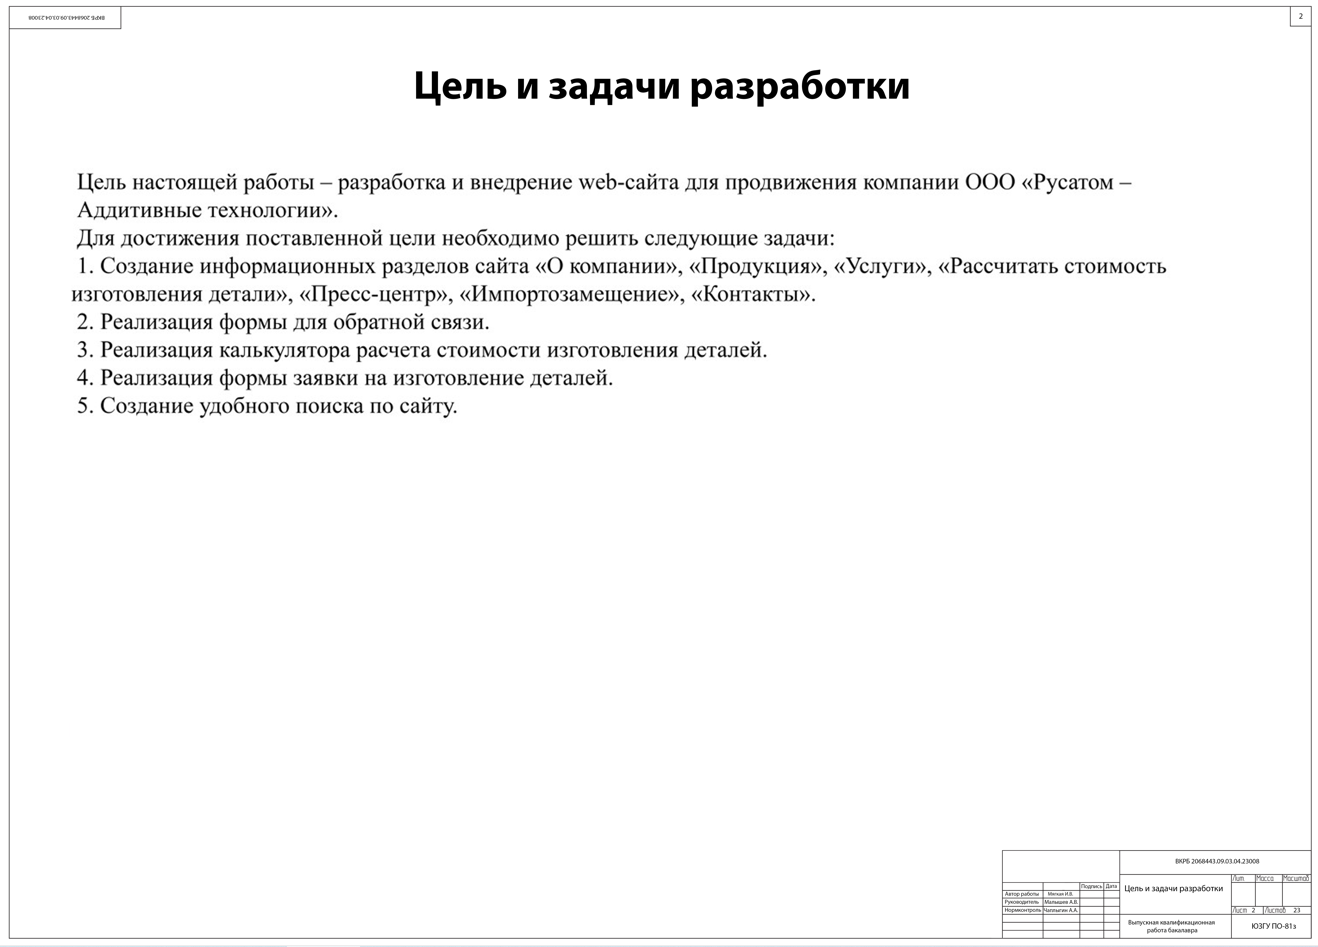
\includegraphics[width=0.82\linewidth]{плакат2.png}
    \заголовок{Цель и задачи разработки}
    \label{pl2:image}      
\end{плакат}

\begin{плакат}
    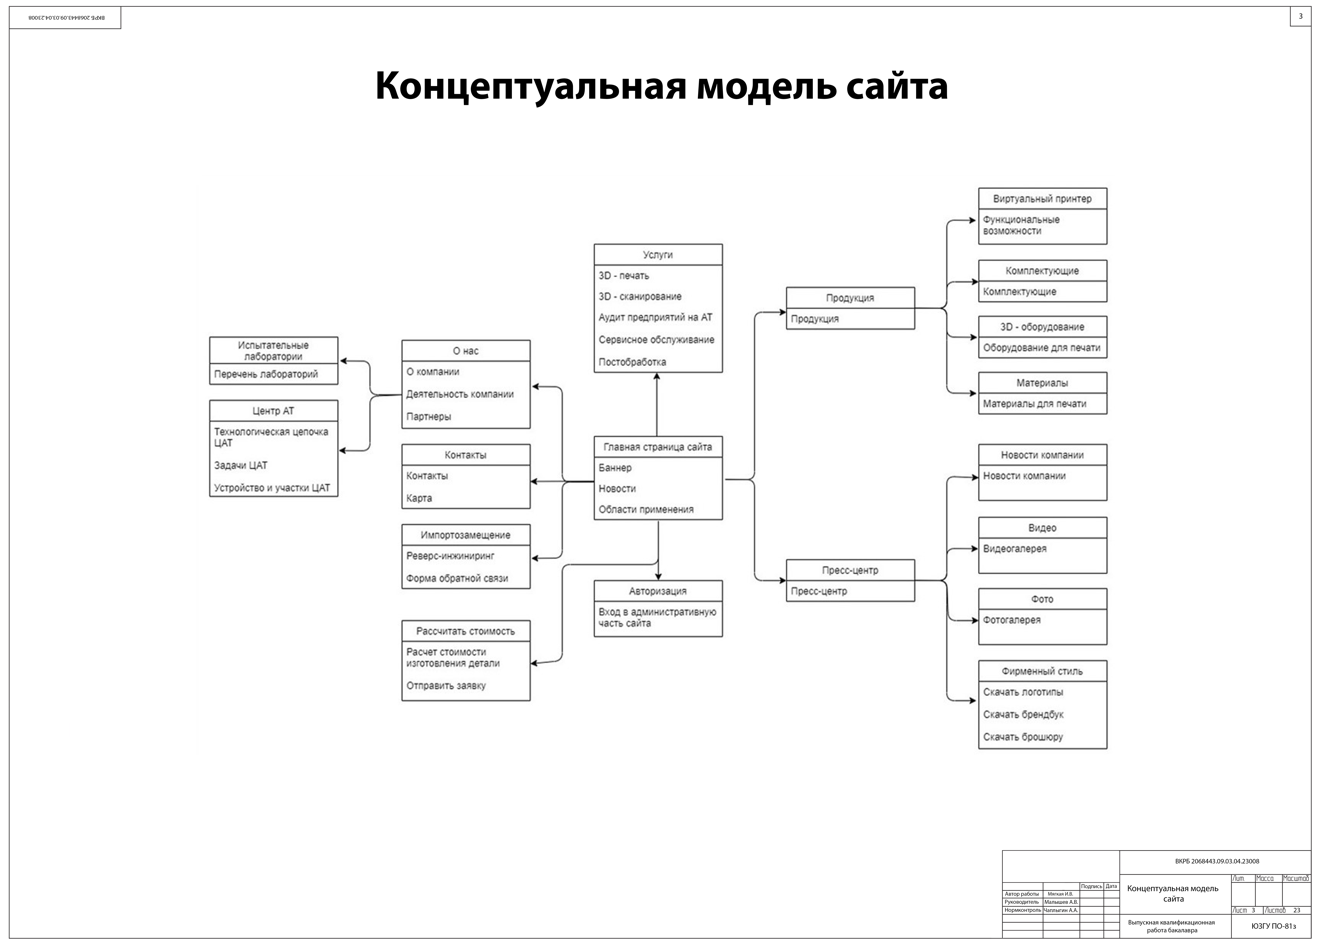
\includegraphics[width=0.82\linewidth]{плакат3.png}
    \заголовок{Концептуальная модель сайта}
    \label{pl3:image}      
\end{плакат}

\begin{плакат}
    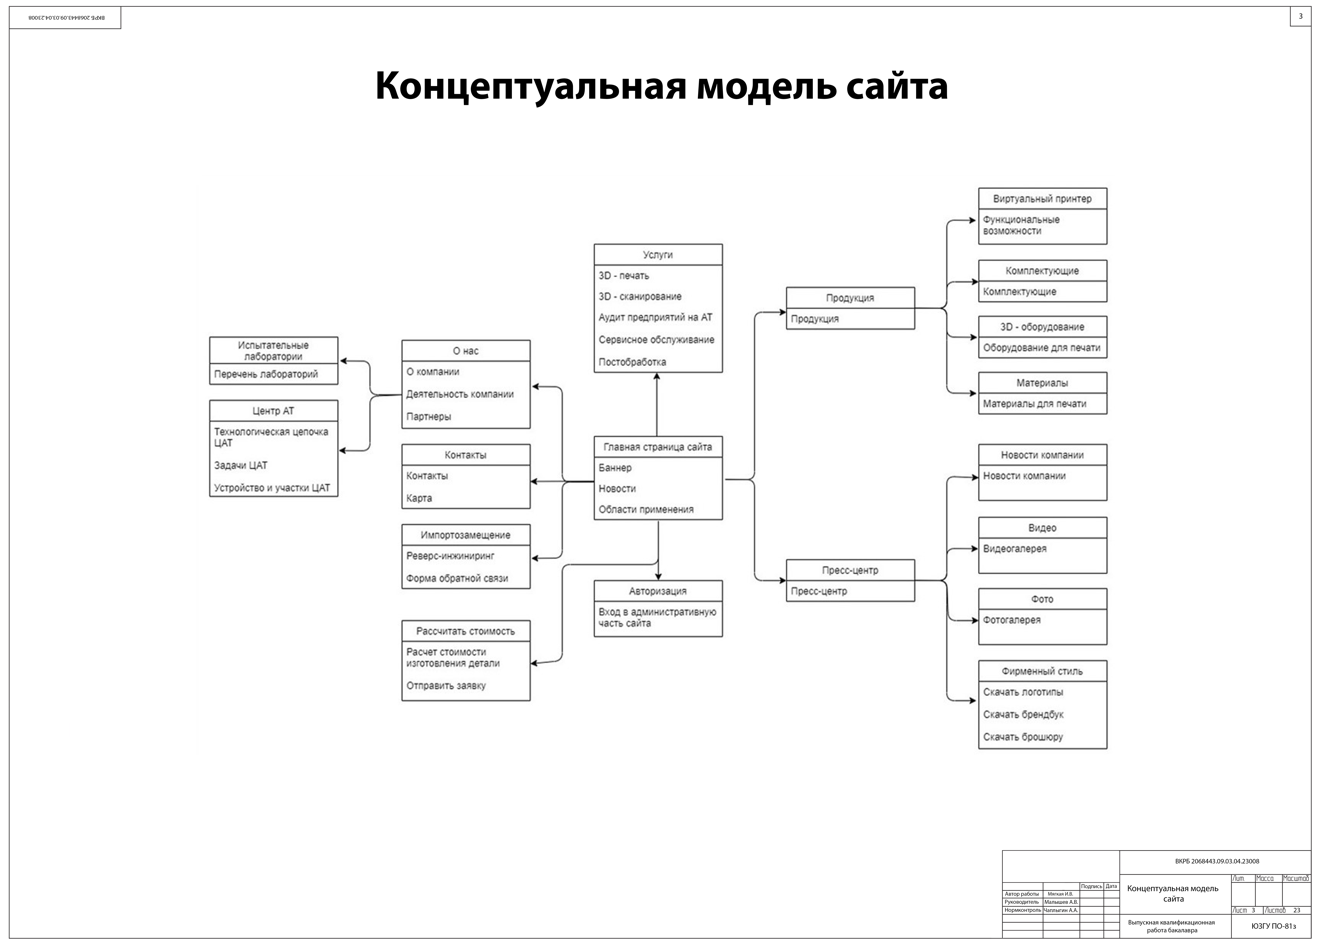
\includegraphics[width=0.82\linewidth]{плакат3.png}
    \заголовок{Еще плакат}
    \label{pl4:image}      
\end{плакат}

\end{landscape}
}\fi
\ifПрактика{}\else{\appendix{Фрагменты исходного кода программы}

main.tex
\lstinputlisting[language=Tex, frame=none]{main.tex}

ТехПроект.tex
\lstinputlisting[language=Tex, frame=none]{ТехПроект.tex}

\ifВКР{
\newpage
\addcontentsline{toc}{section}{На отдельных листах (CD-RW в прикрепленном конверте)}
\noindent
\begin{tabular}{p{5.8cm}C{4.8cm}C{4.8cm}}
   Автор ВКР & \lhrulefill{\fill} & \fillcenter\Автор \\
            \setarstrut{\footnotesize}
           & \footnotesize{(подпись, дата)} & \\
            \restorearstrut
   Руководитель ВКР & \lhrulefill{\fill} & \fillcenter\Руководитель \\
            \setarstrut{\footnotesize}
           & \footnotesize{(подпись, дата)} & \\
            \restorearstrut
   Нормоконтроль & \lhrulefill{\fill} & \fillcenter\Нормоконтроль \\
            \setarstrut{\footnotesize}
           & \footnotesize{(подпись, дата)} & \\
            \restorearstrut
\end{tabular}
\vskip 2cm
\begin{center}
\textbf{Место для диска}
\end{center}
}\fi
}\fi
\end{document}
